% Template for a Computer Science Tripos Part II project dissertation
\documentclass[12pt,a4paper,twoside,openright]{report}
\usepackage[backend=biber]{biblatex}
\usepackage[pdfborder={0 0 0}]{hyperref}    % turns references into hyperlinks
\usepackage[margin=25mm]{geometry}  % adjusts page layout
\usepackage{parskip}
\usepackage{graphicx}  % allows inclusion of PDF, PNG and JPG images
\usepackage{verbatim}
\usepackage{docmute}   % only needed to allow inclusion of proposal.tex
\usepackage{setspace}
\usepackage{amsfonts}
\usepackage{tikz}
\usepackage{float}
\usepackage{amsmath}
\usepackage{bm}
\usepackage{algorithm}
\usepackage[noend]{algpseudocode}
\usepackage{amsthm}
\usepackage{subcaption}
\usepackage{url}
\usepackage[justification=centering]{caption}
\usepackage[utf8]{inputenc}    % utf8 support       %!!!!!!!!!!!!!!!!!!!!
\usepackage[T1]{fontenc}
\usepackage{booktabs}
\addbibresource{references.bib}
 
\usetikzlibrary{arrows,backgrounds}
\usetikzlibrary{positioning}
\usetikzlibrary{decorations.pathreplacing}
\usetikzlibrary{arrows}
\usetikzlibrary{backgrounds}
\tikzstyle{place}=[circle, draw=black, minimum size = 8mm]
\tikzset{>=latex}
\usepgflibrary{shapes.multipart}


\raggedbottom                           % try to avoid widows and orphans
\sloppy
\clubpenalty1000%
\widowpenalty1000%

\renewcommand{\baselinestretch}{1.1}    % adjust line spacing to make
                                        % more readable
\renewcommand{\vec}[1]{\bm{#1}}
\renewcommand{\thealgorithm}{\arabic{chapter}.\arabic{algorithm}}
\newtheorem*{defn}{Definition} 

\begin{document}

%%%%%%%%%%%%%%%%%%%%%%%%%%%%%%%%%%%%%%%%%%%%%%%%%%%%%%%%%%%%%%%%%%%%%%%%
% Title

\pagestyle{empty}

\rightline{\LARGE \textbf{Charles London}}

\vspace*{60mm}
\begin{center}
\Huge
\textbf{A tool for prediction of phenotype from cell genotype} \\[5mm]
{\setstretch{0.5}\Large Alternate: Semi-supervised learning with autoencoders for classification of gene expression data} \\[5mm]
Computer Science Tripos -- Part II \\[5mm]
Trinity College \\[5mm]
\today  % today's date
\end{center}

%%%%%%%%%%%%%%%%%%%%%%%%%%%%%%%%%%%%%%%%%%%%%%%%%%%%%%%%%%%%%%%%%%%%%%%%%%%%%%
% Proforma, table of contents and list of figures

\pagestyle{plain}

\chapter*{Proforma}

{\large
\begin{tabular}{ll}
Name:               & \bf Charles London                      \\
College:            & \bf Trinity College                     \\
Project Title:      & \bf A tool for phenotype prediction from cell genotype  \\
Examination:        & \bf Computer Science Tripos -- Part II, March 2019  \\
Word Count:         & \bf 1587\footnotemark[1]  \\
Project Originator: & Prof P.~Li\'o                   \\
Supervisors:         & Prof P.~Li\'o \& Helena Andres Terre                   \\ 
\end{tabular}
}
\footnotetext[1]{This word count was computed
by \texttt{detex diss.tex | tr -cd '0-9A-Za-z $\tt\backslash$n' | wc -w}
}
\stepcounter{footnote}

\section*{Original Aims of the Project}

\section*{Work Completed}

All that has been completed appears in this dissertation.

\section*{Special Difficulties}

Learning how to incorporate encapulated postscript into a \LaTeX\
document on both Ubuntu Linux and OS X.
 
\newpage
\section*{Declaration}

I, [Name] of [College], being a candidate for Part II of the Computer
Science Tripos [or the Diploma in Computer Science], hereby declare
that this dissertation and the work described in it are my own work,
unaided except as may be specified below, and that the dissertation
does not contain material that has already been used to any substantial
extent for a comparable purpose.

\bigskip
\leftline{Signed [signature]}

\medskip
\leftline{Date [date]}

\tableofcontents

\listoffigures

\newpage
\section*{Acknowledgements}

%%%%%%%%%%%%%%%%%%%%%%%%%%%%%%%%%%%%%%%%%%%%%%%%%%%%%%%%%%%%%%%%%%%%%%%
% now for the chapters

\pagestyle{headings}

\chapter{Introduction}

\textit{The stated aim of this project was to develop a semi-supervised autoencoder-based method for classifying 
cells into phenotypes \footnote{The observable characteristics and traits of an organism} using genetic data. To this end a range 
of autoencoder based semi-supervised models have been implemented, 
ranging from fairly simple to state-of-the-art. These models were then evaluated on selected gene expression datasets, including 
the Cancer Genome Atlas expression data.}

\section{Motivation}

Gene expression is the process of synthesising proteins from the gene via RNA. A transcriptome is the set of all RNA 
molecules in a cell or population of cells. While every cell with a nucleus in an organism has the same DNA and genes, the cells
differ in function, and this depends on which genes are being actively expressed. This in turn means the
transcriptome contains information from both genetic and epigenetic sources~\cite{Gibney2010}. Epigenetic differences are differences
in the phenotype without alterations to the DNA (e.g. DNA methylation). Therefore, as this project aims to classify cells into phenotypes, 
gene expression data is used.

Biological labs worldwide perform transcriptome analysis, resulting in huge amounts of gene expression data being
generated. Much of this is shared or available online, giving researchers access to huge amounts of data. The development
of RNA-Seq using next generation sequencing has also resulted in increased amounts of gene expression data, being more 
accurate and cost effective than previous methods. However,
while many of the datasets generated in different experiments may include transcriptomes for the same species of organism,
the majority of the time the experiments are measuring different phenotypes of the organism. This means that a 
researcher wanting to analyse or predict a specific phenotype is unable to use much of the available data, being limited
to only those labelled with the desired phenotype.

Semi-supervised learning attempts to leverage unlabelled data to improve the accuracy of the machine learning
algorithm on a supervised task. Autoencoders have a long history of being used in semi-supervised learning problems,
having been used early on to improve deep networks by pretraining them using stacked denoising autoencoders (Section~\ref{sdae})
and recently having been used to achieve state of the art semi-supervised performance as part of the ladder 
network (Section~\ref{ladder}). The main reason for their use is that autoencoders are good at learning 
important features of data in an unsupervised manner, and these features are often useful in improving 
supervised performance.

Therefore, with the use of semi-supervised autoencoder models it should be possible to leverage the data without
the desired phenotype to improve performance in predicting the phenotype.

The reason for choosing autoencoder-based models to use with gene expression data is that they are implemented
using neural networks. This is advantageous because neural networks work very well on non-linear data and are
also able to effectively analyse data with very high dimensionality (number of features). Transcriptomes can
often contain several thousand genes, and so any model used must be able to cope with this level of dimensionality.

\section{Related work}

Stacked denoising autoencoders have previously been used with gene expression data to derive the most informative
genes for distinguishing between healthy and cancerous cells~\cite{8217828}.

Likewise, variational autoencoders (Section~\ref{vae}) have been successfully used to extract a biologically relevant latent 
space from cancer transcriptomes ~\cite{Way2018ExtractingAB}. They and the semi-supervised variant (Section~\ref{ssVAE}) 
have also been used to model the change in the gene expression of tumours in response to certain drugs~\cite{10.1093/bioinformatics/btz158}.
he semi-supervised model in the paper, Dr.VAE, jointly models both the drug response and the treatment outcomes.

Ladder networks have also been used in biologically relevant ways, achieving state of the art accuracy in the binary cancer classification
problem using gene expression data~\cite{10.1007/978-3-319-78723-7_23}.

\chapter{Preparation}

\section{Neural networks}

This project involves using \textbf{autoencoders} as a basis for semi-supervised learning and classification of gene expression data. 
Autoencoder architectures are all based on \textbf{deep feedforward networks} so it is important to have a good understanding of the basic principles
of these networks.

\subsection{The perceptron}

The perceptron (also known as the \textbf{artificial neuron}~\cite{WhatareA61:online}) is the basic element of the neural network. It takes in inputs $(x_1, ..., x_n)$ and 
multiplies these by \textbf{weights} $(w_1, ..., w_n)$, giving a linear combination of the inputs $x_1w_1 + ... + x_nw_n$, before applying 
an \textbf{activation function} $\sigma$~\cite{Art_Int}.

It can be helpful to think of the inputs and weights as 
vectors $\vec{x}$ and $\vec{w}$, giving the combination as $\vec{x} \cdot \ \vec{w}$. A \textbf{bias} term $x_0=1$ may also be included and multiplied by 
weight $w_0$, giving $\vec{x} = [1, x_1, ..., x_n]$ and $\vec{w} = [w_0, w_1, ..., w_n]$. Intuitively the bias can be thought of as the intercept
on a graph - if the neuron should have an output when all the inputs are zero it will be unable to model this correctly without a bias.

The function computed by the neuron is then:
\begin{equation}
  y = \sigma(\vec{x} \cdot \vec{w})
\end{equation}

\begin{figure}[H]
  \begin{center}
      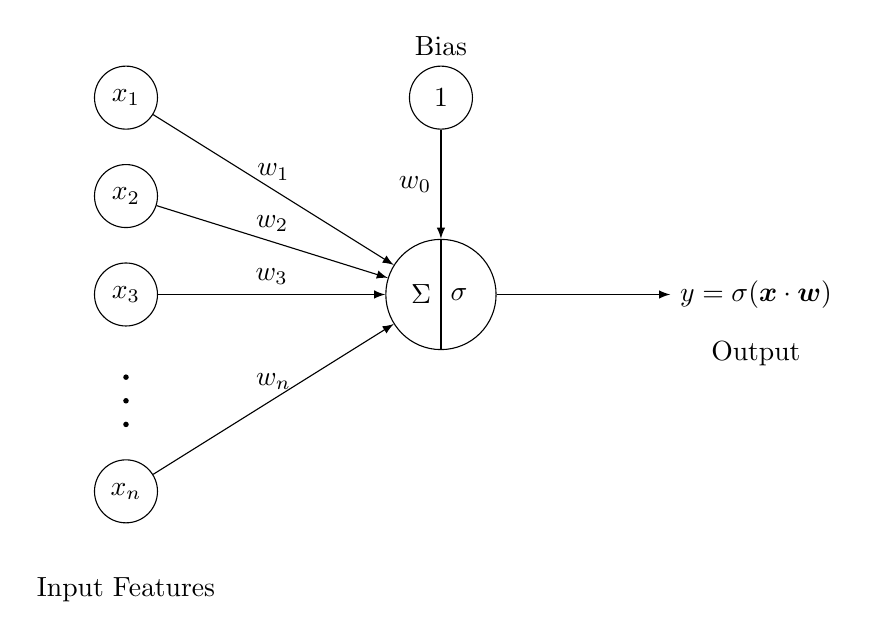
\begin{tikzpicture}
        \tikzstyle{place}=[circle, draw=black, minimum size = 8mm]
        
         % Output
         \node at (4, -3*1.25) [circle split, draw=black, minimum size = 14mm, rotate=90] (out) 
         {\rotatebox{-90}{$\Sigma$} \nodepart{lower} \rotatebox{-90}{$\sigma$}};

        % Input
        \foreach \x in {1,...,3}
          \draw node at (0, -\x*1.25) [place] (input_\x) {$x_\x$};
        \foreach \x in {1,...,3}
          \fill (0, -4.5 -\x*0.3) circle (1pt);
        \draw node at (0, -5*1.25) [place] (input_n) {$x_n$};

        % Bias
        \node at (4, -1.25) [place] [label={Bias}] (bias) {$1$};

        % Function
        \node at (8, -3*1.25) [] (func) {$y = \sigma(\vec{x} \cdot \vec{w})$};

        % Bias -> Out
        \draw [->] (bias) -- (out) node [left, midway] {$w_0$};
          
        % Input -> Out
        \foreach \i in {1,...,3}
          \draw [->] (input_\i) -- (out) node [above, midway] {$w_\i$};
        \draw [->] (input_n) -- (out) node [above, midway] {$w_n$};
        \path[->] (out) edge node[] {} (func);
        
        % Text
        \node at (0, -7.5) [black, ] {Input Features};
        \node at (8, -4.5) [black, ] {Output};
      \end{tikzpicture}
      \caption{A perceptron}
      \label{fig:illustration_perceptron}
  \end{center}
\end{figure}

The activation function applied will depend on what the neuron is being used for.
Some common activation functions and their uses are~\cite{Art_Int}:
\begin{itemize}
  \item \textbf{Linear}
        \begin{equation}
          \sigma(z) = z
        \end{equation}
        Used in regression problems, when a real-valued output that can take any value is required.
  \item \textbf{Sigmoid}
        \begin{equation}
          \sigma(z) = \frac{1}{1 + e^{-z}}
        \end{equation}
        Used to give output values in the range $[0,1]$, for example to give a probability of a class in binary classification (two classes).
        Was previously used as the non-linear function in hidden layers but has seen reduced usage with the increased popularity of ReLU.
  \item \textbf{ReLU}
        \begin{equation}
          \sigma(z) = max(0, z)
          \label{eq:relu}
        \end{equation}
        Used in the hidden layers of deep feedforward networks (described in the next section) to provide non-linearity, allowing the network to learn more 
        complicated functions. Has seen massive uptake due to performance benefits over sigmoid~\cite{relu}.
\end{itemize}

\subsection{Deep feedforward networks}

Deep feedforward networks are made up of multiple perceptrons arranged into \textbf{layers} (and are often called multilayer perceptrons). 
Each neuron in a layer has its own set of weights
$\vec{w}$ and takes the ouputs of the previous layer (or the inputs to the network if the neuron is in the first layer) $\vec{x}$ in order to compute the 
output value $y$ for the neuron. This value is then used as an input to the next layer, or part of the output of the network if the neuron is in
the output layer. (N.B. I will use the terms deep feedforward network and neural network interchangably).
\begin{figure}[H]
  \begin{center}
      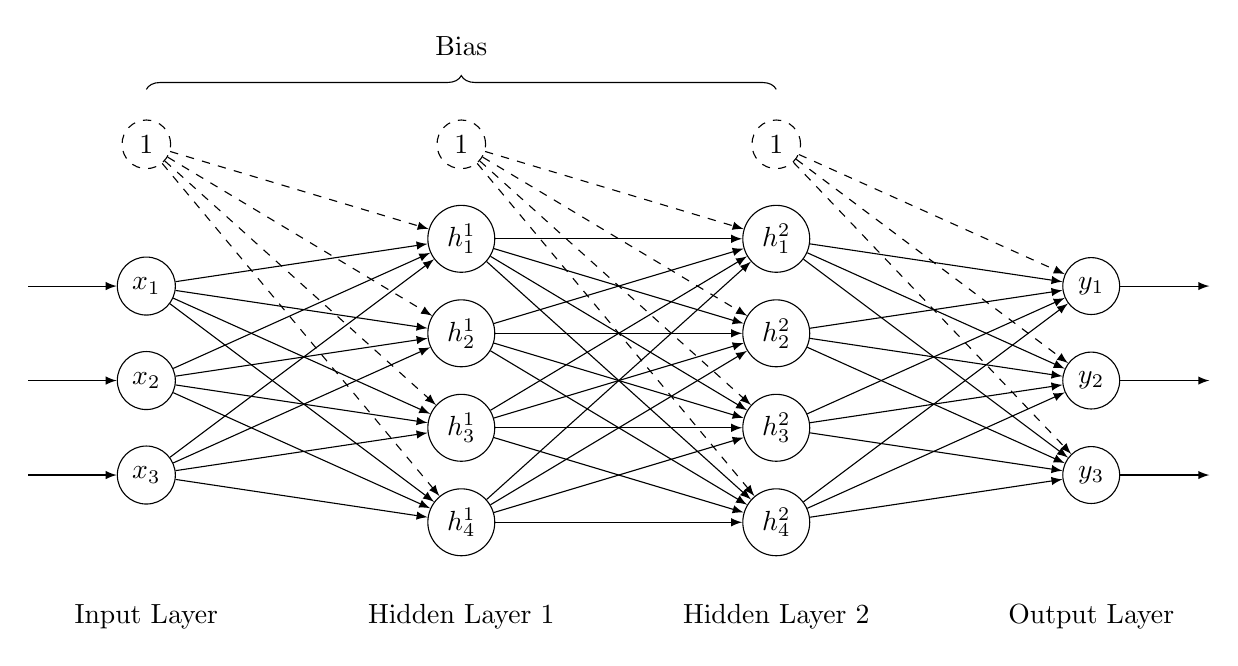
\begin{tikzpicture}
        \tikzstyle{place}=[circle, draw=black, minimum size = 4mm]
        
        % Input
        \draw node [dashed] at (0, 0) [place] (first_0) {$1$};
        \foreach \x in {1,...,3}
          \draw node at (0, -\x*1.2 - 0.6) [place] (first_\x) {$x_\x$};
        \foreach \x in {1,...,3}
          \draw [->] (-1.5, -\x*1.2 - 0.6) to (first_\x); 
        
        % Hidden 1
        \draw node [dashed] at (4, 0) [place] (second_0) {$1$};
        \foreach \x in {1,...,4}
          \node at (4, -\x*1.2) [place] (second_\x) {$h^{1}_\x$};

        % Hidden 2
        \draw node [dashed] at (8, 0) [place] (third_0) {$1$};
        \foreach \x in {1,...,4}
          \node at (8, -\x*1.2) [place] (third_\x) {$h^{2}_\x$};
        
        % Output
        \foreach \x in {1,...,3}
          \node at (12, -\x*1.2 - 0.6) [place] (fourth_\x) {$y_\x$};
        \foreach \x in {1,...,3}
          \draw [->] (fourth_\x) to (13.5, -\x*1.2 - 0.6); 

        \draw [decorate,decoration={brace,amplitude=5pt,raise=-2ex}]
          (0,1) -- (8,1) node[above,midway]{Bias};
          
        % Input -> Hidden 1
        \foreach \i in {1,...,4}
          \draw [->,dashed] (first_0) to (second_\i);
        \foreach \i in {1,...,3}
          \foreach \j in {1,...,4}
            \draw [->] (first_\i) to (second_\j);
        
        % Input -> Hidden 2
        \foreach \i in {1,...,4}
          \draw [->,dashed] (second_0) to (third_\i);
        \foreach \i in {1,...,4}
          \foreach \j in {1,...,4}
            \draw [->] (second_\i) to (third_\j);
        
        % Hidden -> Output
        \foreach \i in {1,...,3}
          \draw [->,dashed] (third_0) to (fourth_\i);
        \foreach \i in {1,...,4}
          \foreach \j in {1,...,3}
            \draw [->] (third_\i) to (fourth_\j);
        
        % Text
        \node at (0, -6) [black, ] {Input Layer};
        \node at (4, -6) [black, ] {Hidden Layer 1};
        \node at (8, -6) [black, ] {Hidden Layer 2};
        \node at (12, -6) [black, ] {Output Layer};
      \end{tikzpicture}
      \caption{Illustration of a 4-layer deep feedforward network}
      \label{fig:illustration_deep_network}
  \end{center}
\end{figure}

The primary source of the following information is \textit{Deep Learning} by Goodfellow et al.~\cite{Goodfellow-et-al-2016}. 
The naming convention \textbf{deep} comes about because the networks contain multiple layers. Deep is usually used to refer to networks 
with multiple hidden layers. \textbf{Feedforward} comes from the fact that information 
in the network flows forward from layer to layer, with no connections allowing the information to move backwards to previous layers.

The main reason for neural networks with multiple layers is that they can model much more \textbf{complex non-linear relationships} than single 
neurons and single layer models are able to. Using non-linear activation functions such as ReLU \eqref{eq:relu} allow neurons to model simple 
non-linear functions, and combining these into layers allows them to model these more complex non-linear relationships.

I will denote the function computed by a neural network as $f_{\vec{\theta}}(\vec{x})$, where $\vec{\theta}$ denotes the trainable parameters of the neural
network (in the simplest case the weights).

\subsection{Supervised learning}

There are two main problems that neural networks are usually used to solve: \textbf{regression} and \textbf{classification}~\cite{ML_Bayes}:
\begin{itemize}
  \item Regression problems involve predicting the value of a quantity that is continuous and real-valued: $f_{\vec{\theta}}(\vec{x}) \in \mathbb{R}$. 
  \item Classification problems involve predicting which class (of a pre-determined set) an input belongs to: $f_{\vec{\theta}}(\vec{x}) \in [l_0,...,l_n]$.
\end{itemize}

Supervised learning involves taking a \textbf{dataset} $s=((\vec{x_0}, y_0),...,(\vec{x_n}, y_n))$ and using that to train a network to find a function 
that gives good predictions for $y$ given $\vec{x}$: $f_{\vec{\theta}}(\vec{x}) = \hat{y} \approx y$.

\subsubsection{Neural networks for classification}
This project has focused exclusively on classification problems, and so a more in-depth description is necessary.

A dataset for classification training is given as pairs of numerical \textbf{features} and a \textbf{label}: $(\vec{x}, y)$. These features are the input to our network,
and the label is our target. A label cannot be directly utilised by the a neural network as they operate on numerical data. Therefore it is 
necessary to transform the data into a numerical representation.

\textbf{One-hot encoding} assigns an integer $i$ to each class and makes a vector of length $n$ (where $n$ is the 
number of classes), setting the $ith$ element to one and all other elements to zero. For example, with three classes, red, green, and blue
the one hot labels would be $[1, 0, 0]$ , $[0, 1, 0]$ and $[0, 0, 1]$. The network then has an output node corresponding to each class.
This provides no implicit ordering over the classes (a problem found in integer coding) as each output node is equally important to the 
network \cite{WhyOneHo55:online}.

The output from the network is then a real number for each class. This does not lend itself easily to a loss function (more explanation
in next section) and can also be difficult to interpret for humans. Therefore the \textbf{softmax} function is used as the activation function
in the ouput layer:
\begin{align} \label{softmax}
  \sigma(y_j) = \frac{e^{y_j}}{\sum_{i=1}^{K} e^{y_i}},  &\text{ for the $jth$ output in K output values}
\end{align}

This give a value in the range $[0,1]$ for every class, the sum of which is $1$. It is now possible to view the output of the model as a 
probability distribution over the classes~\cite{10.1007/978-3-642-76153-9_28}, which allows the model to encode uncertainty and is easily interpretable by humans. It also lends 
itself well to a loss function.

\subsection{Training the network}

Neural networks usually have their weights initialised to small random values. This means that on the first pass
the output of the network will likely be very far from the correct value. The difference between the correct
value and the network output is called the \textbf{loss}. Training a neural network involves adjusting its
trainable parameters ($\vec{\theta}$) until the network reaches an acceptable loss or accuracy. This is done by computing
a loss function, which measures how well a neural network is performing on the training set, and updating the parameters to decrease the loss.

\subsubsection{Loss functions}

The two main loss functions used in this project are \textbf{mean square error} and \textbf{cross entropy} loss:
\begin{itemize}
  \item \textbf{Mean square error}
        \begin{align}
          J(\vec{\theta}) = \frac{1}{n}\sum_{i=1}^{n} (f_{\vec{\theta}}(\vec{x}^i) - y^i)^2 \label{eq:mse}
        \end{align}
        The mean square error is the mean of the squared difference between the real values and the 
        predicted values for multiple datapoints. If the output from the network and the correct values are 
        vectors it is calculated by taking the Euclidean distance between them ($|f_{\vec{\theta}}(\vec{x}^i) - \vec{y}^i|^{2}$) 
        and squaring it. This loss function is defined for all real numbers and so is used in regression problems. 
        It is also used as the reconstruction loss in most of the autoencoders in this project.
  \item \textbf{Cross entropy}
        \begin{align}
          J(\vec{\theta}) = - \frac{1}{n}\sum_{i=1}^{n} \vec{y}^i \cdot \log{f_{\vec{\theta}}(\vec{x}^i)} \label{eq:ce}
        \end{align}
        This loss function is used for multiclass classification problems. $\vec{y}^i$ is the one-hot 
        representation of the label, and the scalar product is taken with the logarithm of the softmax output 
        probabilities. This comes out to $\log{f_{\vec{\theta}}(\vec{x}^i)_j}$ where the $jth$ label is the correct one.
        Taking the negative of this means that if the probability of the correct label is high then the loss is 
        very low ($\lim_{x \to 1} -\log{x} = 0$) and if the probability is low then the loss is very high 
        ($\lim_{x \to 0} -\log{x} = \infty$).
\end{itemize}

\subsubsection{Updating the weights}

Forward propagation is the flow of information through the network from input features to the output values. From these output values the loss is calculated. 
The trainable parameters of a neural network can then be updated by first finding the gradient of the loss with respect to these trainable parameters.
The process of computing these gradients is called \textbf{backpropagation} and a full derivation can be found in Appendix~\ref{backprop}. The important notation is:

\begin{itemize}
  \item $\theta$ is a vector of all the trainable parameters in the network
  \item $J(\vec{\theta})_k$ is the loss for the $kth$ sample in the training set
  \item $\nabla_{\vec{\theta}} J(\vec{\theta})_k$ is a vector of gradients of the loss with respect to all the trainable parameters 
\end{itemize}

Once the gradients for all the weights have been calculated the weights are updated. By moving the weights a small step in the direction of steepest 
negative gradient the loss should decrease as the parameters are shifting it towards a minima. This means that the model is getting 
better at modelling the training set. Taking these small steps is called \textbf{gradient descent}. The weight update rule is: 
\begin{align}
  \vec{\theta} & := \mathbf{\vec{\theta}} - \eta \sum_{k} \frac{\partial J(\vec{\theta})_k}{\partial \mathbf{\vec{\theta}}} \\
  & := \mathbf{\vec{\theta}} - \eta \sum_{k} \nabla_{\vec{\theta}} J(\vec{\theta})_k \\
  & := \mathbf{\vec{\theta}} - \eta \nabla_{\vec{\theta}} \sum_{k} J(\vec{\theta})_k \label{eq:weight}
\end{align}

$\eta$ is a \textbf{hyperparameter}. Hyperparameters are parameters of the model that are not trained but are set by the user before training.
$\eta$ is called the \textbf{learning rate} and controls how large of a step is taken each time the weight is updated. If the learning rate is 
too high the weights can ``jump" over minima, and even diverge out of a minima, but if the rate is too low it can take too long to converge,
or get stuck in a less desirable local minima. The step size is also proportional to the magnitude of the gradient, allowing the optimizer to 
take a larger step towards a minima if the gradient is steeper

The basic form of gradient descent outlined above uses one constant learning rate ($\eta$) for updating all
of the weights in the network. Recently most neural network implementations have instead used \textbf{Adam}, an adaptation of gradient descent that holds
a learning rate per trainable parameter, and updates this based on the mean and variance of the gradients.

\subsubsection{Batch learning}

The reason for including a summation term over training set samples in both the loss functions (\eqref{eq:mse} \& \eqref{eq:ce}) and the weight update rule \eqref{eq:weight}
is because neural networks are generally run over multiple samples each time they are run, rather than being run over a single example. When performing gradient descent there
are three main ways:
\begin{itemize}
  \item \textbf{Stochastic} gradient descent is computed over a single sample per iteration.
  \item \textbf{Mini-batch} gradient descent uses multiple samples per iteration, but less than the whole dataset.
  \item \textbf{Batch} gradient descent uses the entire dataset per iteration
\end{itemize}

The most popular of these approaches is mini-batch, as it has stability advantages over stochastic and computational advantages over batch. Stochastic gradient
descent has more noise as each update is based on an individual example, causing the weights to jump around more. It also doesn't take advantage of the 
parallelisation possiblity of much hardware - it's much more efficient to send multiple sampels through at once. Batch has the problem of storing the whole 
dataset in memory, and only making one update per pass through the dataset can mean the model takes longer to converge to the best parameters. Mini-batch manages to
have less noise than stochastic due to averaging over multiple samples, while also taking advantage of parallelisation and not requiring huge amounts of memory.

\subsubsection{Summary}

One complete pass through the dataset is called an \textbf{epoch}. Training involves running forward and backpropagation for a certain number of epochs to minimise the loss
on the training set and cause the model to converge to a good approximation to the real function. The pseudocode for training the network is shown below.
\begin{algorithm}
  \begin{algorithmic}[1]
    \Procedure{Training}{$i$, $\mathcal{D}$, $\eta$, \texttt{model}, \texttt{loss\char`_function}}
    \For{$i$ epochs}
    \For{mini-batch $\mathcal{M}$ in $\mathcal{D}$}
    \State \texttt{data, labels} = $\mathcal{M}$
    \State \texttt{out} = \texttt{model(data)}
    \State $\mathcal{J}$ = \texttt{loss\char`_function(out, labels)}
    \State \texttt{model}.$\vec{\theta}$ = \texttt{model}.$\vec{\theta}$ - $\eta \nabla_{\vec{\theta}} \mathcal{J}$ 
    \EndFor
    \EndFor
    \EndProcedure
  \end{algorithmic}
  \caption{Train neural network via mini-batch gradient descent} 
  \label{alg:train}
\end{algorithm}

\section{The manifold hypothesis}

The \textbf{dimensionality} of data is the number of features needed to specify the data. For example, a very popular machine learning dataset
is the MNIST dataset, containing 28x28 grayscale images of handwritten digits. The dimensionality of each datapoint is 784, as that is the
number of pixels specifying each image.

\textbf{The manifold hypothesis} suggest that high dimensional data can actually be viewed as lying on or near to a
lower dimensional manifold embedded in this higher dimensional space.

The precise definition of an n-dimensional manifold is ``a 
topological space that is locally Euclidean", i.e. there is a neighbourhood around each point on the manifold that can be describe as n-dimensional 
Euclidean space. However, it is much easier to think about with an intuitive example - imagine that all the datapoints in a 
dataset lie on piece of paper, and so can be described with two features, an $x$ and $y$ axis. If the paper is taken and scrunched up and 
twisted it now has a three dimensional shape, but the data still lies on a two-dimensional manifold and, by unscrunching the paper, can still 
be described with only two features.
\begin{figure}[H]
  \centering
  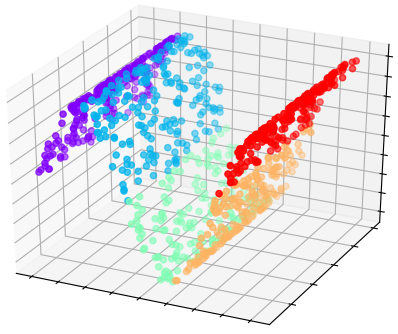
\includegraphics[width=8cm]{figs/manifold.png}
  \caption{Points on a 2-dimensional manifold embedded in 3-dimensional space}
  \label{fig:manifold}
\end{figure}

Therefore, what the manifold hypothesis is suggesting is that many features in high dimensional data are actually redundant,
and the data can be described using fewer features. Again this can be seen intuitively by the fact that the set of 784 pixel images 
that look like a recognisable digit is a very small subset of the set of 784 pixel images - if the pixel values were selected randomly from 
between 0 and 255 the picture would look like random noise, leading to the conclusion that there is a lot of redundancy in the MNIST features.
\begin{figure}[H]
  \centering
  \begin{subfigure}[b]{0.4\linewidth}
    
\includegraphics[width=\linewidth,scale=1]{figs/rand_noise.png}
    \caption{Pixel values selected randomly}
  \end{subfigure}
  \begin{subfigure}[b]{0.4\linewidth}
    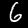
\includegraphics[width=\linewidth,scale=1]{figs/digit.png}
    \caption{MNIST digit}
  \end{subfigure}
  \caption{Demonstrating redundancy of features in MNIST dataset}
  \label{fig:digit}
\end{figure}

The manifold hypothesis then leads to \textbf{non-linear dimensionality reduction} techniques. By finding this lower dimensional
mainfold the data can be explained with fewer features and possibly be more easily seperated and classified. Going back to the paper example,
linear dimensionality reduction techniques (e.g. principal component analysis) would be able to find the 2D embedding if the paper were 
rotated, translated or stretched, but would be unable to unscrunch the paper, as that amounts to a non-liner embedding. Autoencoders are 
used for non-linear dimensionality reduction, and are described in the next section.

\section{Autoencoders}

Autoencoders use neural networks in an unsupervised way to try and learn new \textbf{latent} representations of the data, typically with reduced 
dimensionality (i.e. there are fewer features in the latent data than in the input data). The use of neural networks allow it to learn a 
non-linear mapping from the data to the latent representation, the advantages of which were explained in the previous section.

Autoencoders are made up of two parts, the encoder and the decoder. The encoder takes in the original data, $\vec{x}$, 
and outputs a latent representation, $\vec{z} = f_{\vec{\theta}}(\vec{x})$. The decoder then takes in this latent representation and 
attempts to reconstruct $\vec{x}$, outputting $\vec{\hat{x}} = h_{\vec{\phi}}(\vec{z})$. This allows an unsupervised problem to be turned 
into a supervised problem, using $\vec{x}$ as the target.
\begin{figure}[H]
  \begin{center}
      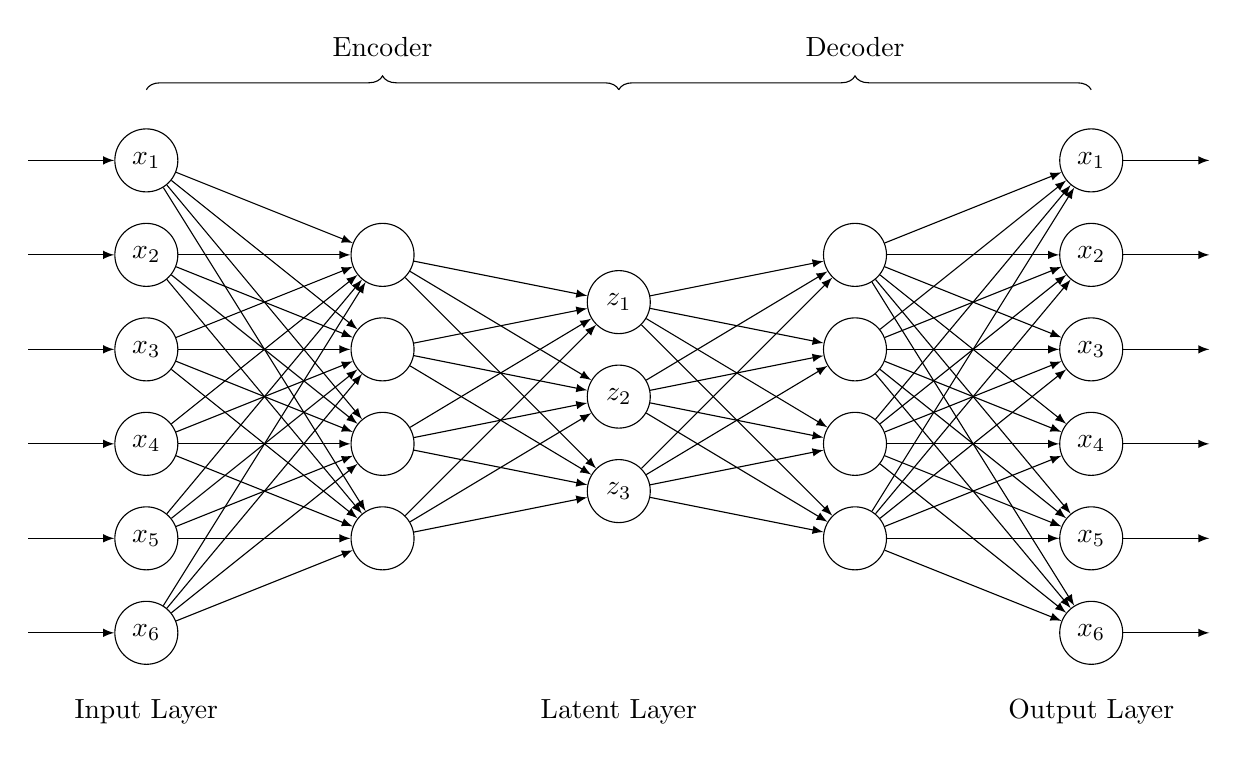
\begin{tikzpicture}
        \tikzstyle{place}=[circle, draw=black, minimum size = 8mm]
        
        % Input
        \foreach \x in {1,...,6}
          \draw node at (0, -\x*1.2) [place] (first_\x) {$x_\x$};
        
        % Hidden 1
        \foreach \x in {1,...,4}
          \node at (3, -1.2 -\x*1.2) [place] (second_\x){};

        % Latent
        \foreach \x in {1,...,3}
          \node at (6, -1.8 -\x*1.2) [place] (third_\x){$z_\x$};

        % Hidden 2
        \foreach \x in {1,...,4}
          \node at (9, -1.2 -\x*1.2) [place] (fourth_\x){};
        
        % Output
        \foreach \x in {1,...,6}
          \draw node at (12, -\x*1.2) [place] (fifth_\x) {$x_\x$};
          
        \foreach \i in {1,...,6}
          \draw [->] (-1.5, -\i*1.2) to (first_\i);

        \foreach \i in {1,...,6}
          \foreach \j in {1,...,4}
            \draw [->] (first_\i) to (second_\j);

        \foreach \i in {1,...,4}
          \foreach \j in {1,...,3}
              \draw [->] (second_\i) to (third_\j);

        \foreach \i in {1,...,3}
          \foreach \j in {1,...,4}
            \draw [->] (third_\i) to (fourth_\j);
        
        \foreach \i in {1,...,4}
          \foreach \j in {1,...,6}
              \draw [->] (fourth_\i) to (fifth_\j);

        \foreach \i in {1,...,6}
          \draw [->] (fifth_\i) to (13.5, -\i*1.2);

        \draw [decorate,decoration={brace,amplitude=5pt,raise=-2ex}]
          (0,0) -- (6,0) node[above,midway]{Encoder};
        \draw [decorate,decoration={brace,amplitude=5pt,raise=-2ex}]
          (6,0) -- (12,0) node[above,midway]{Decoder};
        
        % Text
        \node at (0, -8.2) [black, ] {Input Layer};
        \node at (6, -8.2) [black, ] {Latent Layer};
        \node at (12, -8.2) [black, ] {Output Layer};
      \end{tikzpicture}
      \caption{Illustration of a simple autoencoder}
      \label{fig:illustration_autoencoder}
  \end{center}
\end{figure}

\subsection{Simple autoencoders}

Simple autoencoders, as in the figure above, constrain the network by making the number of latent features smaller than the number of input
features. This prevents the network from simply learning the identity function, and hopefully results in an informative latent space.

\subsubsection{Training}
Autoencoders can be trained end to end using backpropagation as explained in section \ref{backprop}. In order to do this they need a loss
function, and the simplest and most widely used is MSE loss \eqref{eq:mse}. The target $x$ and output $\hat{x}$ are both vectors and so 
the Euclidean distance is used as the loss per datapoint. Both the encoder weights $\theta$ and decoder weights $\phi$ are trained at the 
same time; the gradients are backpropagated through the decoder to the latent layer and then back through the encoder every iteration. 

\subsection{Denoising autoencoders}

Denoising autoencoders corrupt the input data with noise (e.g. by adding Gaussian noise or setting some of
the features to 0) giving $\tilde{\vec{x}}$, which is then used as the input to the network. However the target is the uncorrupted input data, 
$\vec{x}$. The aim is to force the autoencoder to learn a better set of features because it not only has to reconstruct the data but also 
has to remove the noise. They can be trained in the same way as a simple autoencoder.

Denoising autoencoders were used extensively to pre-train deep neural networks in the early 2010s, but this has become less popular with the 
introduction of new \textbf{non-saturating} activation functions such as ReLU which have helped deal with the vanishing gradient problem
[Appendix ??].

\subsection{Variational autoencoders} \label{vae}

Variational autoencoders are based on Bayesian inference, and differ from other autoencoders in that the encoder outputs
the parameters of a probability distribution over the latent variables, rather than a single configuration. Variational autoencoders were 
introduced by Kingma and Welling in 2013 and have become one of the most popular unsupervised learning techniques.
\begin{figure}[H]
  \begin{center}
      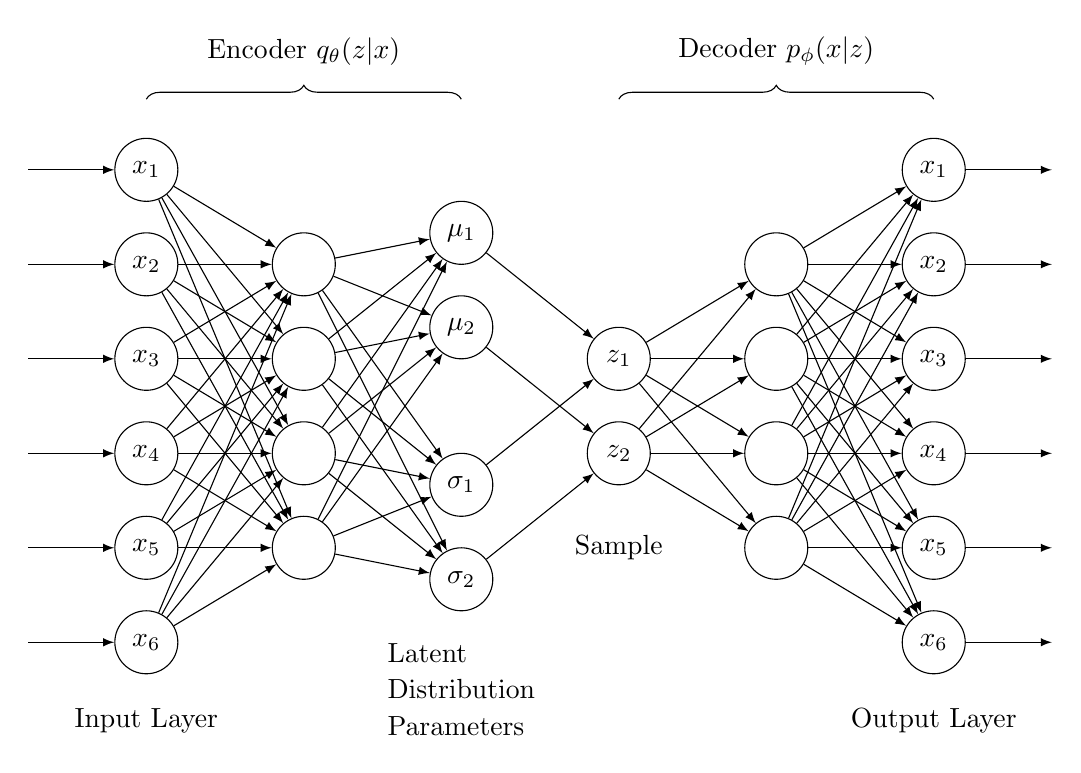
\begin{tikzpicture}
        \tikzstyle{place}=[circle, draw=black, minimum size = 8mm]
        
        % Input
        \foreach \x in {1,...,6}
          \draw node at (0, -\x*1.2) [place] (first_\x) {$x_\x$};
        
        % Hidden 1
        \foreach \x in {1,...,4}
          \node at (2, -1.2 -\x*1.2) [place] (second_\x){};

        % Mu
        \foreach \x in {1,...,2}
          \node at (4, -0.8 -\x*1.2) [place] (mu_\x){$\mu_\x$};

        \foreach \x in {1,...,2}
          \node at (4, -4 -\x*1.2) [place] (logvar_\x){$\sigma_\x$};

        \foreach \x in {1,...,2}
          \draw node at (6, -2.4 -\x*1.2) [place] (sample_\x){$z_\x$};

        % Hidden 2
        \foreach \x in {1,...,4}
          \node at (8, -1.2 -\x*1.2) [place] (fourth_\x){};
        
        % Output
        \foreach \x in {1,...,6}
          \draw node at (10, -\x*1.2) [place] (fifth_\x) {$x_\x$};
          
        \foreach \i in {1,...,6}
          \draw [->] (-1.5, -\i*1.2) to (first_\i);

        \foreach \i in {1,...,6}
          \foreach \j in {1,...,4}
            \draw [->] (first_\i) to (second_\j);

        \foreach \i in {1,...,4}
          \foreach \j in {1,...,2}
              \draw [->] (second_\i) to (mu_\j);
        \foreach \i in {1,...,4}
          \foreach \j in {1,...,2}
            \draw [->] (second_\i) to (logvar_\j);

        \foreach \i in {1,...,2}
          \draw [->] (logvar_\i) to (sample_\i);
        
        \foreach \i in {1,...,2}
          \draw [->] (mu_\i) to (sample_\i);

        \foreach \i in {1,...,2}
          \foreach \j in {1,...,4}
            \draw [->] (sample_\i) to (fourth_\j);
        
        \foreach \i in {1,...,4}
          \foreach \j in {1,...,6}
            \draw [->] (fourth_\i) to (fifth_\j);

        \foreach \i in {1,...,6}
          \draw [->] (fifth_\i) to (11.5, -\i*1.2);

        \draw [decorate,decoration={brace,amplitude=5pt,raise=-2ex}]
          (0,0) -- (4,0) node[above,midway]{Encoder $q_\theta(z|x)$};
        \draw [decorate,decoration={brace,amplitude=5pt,raise=-2ex}]
          (6,0) -- (10,0) node[above,midway]{Decoder $p_\phi(x|z)$};
        
        % Text
        \node at (0, -8.2) [black, ] {Input Layer};
        \node at (4, -7.8) [black, align=left] {Latent \\ Distribution\\ Parameters};
        \node at (6, -6) [black, ] {Sample};
        \node at (10, -8.2) [black, ] {Output Layer};
      \end{tikzpicture}
      \caption{Illustration of a Gaussian variational autoencoder}
      \label{fig:gauss_vae}
  \end{center}
\end{figure}

The central idea of variational autoencoders is that the data $x$ has been generated from some lower dimensional latent
representation $z$. Each datapoint $x_{i}$ is generated by:
\begin{itemize}
  \item sampling $z_{i}$ from the prior distribution over $z$: $z_{i} \sim p(z)$, 
  \item sampling $x_{i}$ from the conditional distribution $p(x|z)$ (known as the likelihood): \\ $x_{i} \sim p(x|z=z_{i})$
\end{itemize}

The prior $p(z)$ can be thought of as constraining the possible space of latent variables. For example, in the MNIST dataset a 
normal autoencoder could place 3s written in different styles in different areas of n-dimensional Euclidean space (where n is the 
dimensionality of $z$) as the latent representation is a vector of unconstrained real numbers. This is detrimental to learning a meaningful 
latent space, and by constraining this space with a prior it should force the model to keep the representations of similar datapoints close.

The decoder of the VAE is a neural network that models the likelihood, $p_\phi(x|z)$. Once the VAE is trained new samples similar to 
those in the training set can be generated by sampling from the prior and passing this into the decoder; this is why VAE's are often
referred to as generative models.

In most situations where unsupervised learning is useful only $x$ is known. The goal is then to infer $z$.
Inference in the model refers to finding good values of the latent variables given the data. This can be done by computing the
posterior, $p(z|x)$. Using Bayes rule we have:
\begin{equation}
  p(z|x) = \frac{p(x|z)p(z)}{p(x)}
\end{equation}

The denominator $p(x)$ is known as the evidence and calculating it is intractable as it has to be computed by marginalizing out $z$:
\begin{equation}
  p(x) = \int p(x|z)p(z) dz
\end{equation}

Computing this integral requires exponential time as it has to be computed over all the possible configurations of
the latent variables. Therefore the posterior is approximated with another simpler distribution $q(z|x)$ defined so that it is 
tractable. The most popular distribution, and the one used in this project, is the Gaussian.
This can then be modelled by a neural network $q_\theta(z|x)$. This is the encoder.

\subsubsection{Training}

The loss function used for a variational autoencoder can be derived by maximizing the probability of the evidence.
This makes sense intuitively, as a good model should maximise the probability of the real data ~\cite{SVIPartI90:online}.
\begingroup
\allowdisplaybreaks
\begin{align*}
  \log p(x) & = \log \int p(x|z)p(z) dz &\text{Law of total probability}\\
  & = \log \int p(x|z)p(z) \frac{q(z|x)}{q(z|x)} dz\\
  & = \log\left(\mathbb{E}_q \left[\frac{p(x|z)p(z)}{q(z|x)}\right]\right) \\
  & \geq \mathbb{E}_q \left[\log\frac{p(x|z)p(z)}{q(z|x)}\right] &\text{Jensen's inequality}\\
  & = \mathbb{E}_q \left[\log p(x|z) + \log\frac{p(z)}{q(z|x)}\right] \\
  & = \mathbb{E}_q [\log p(x|z)] - D_{KL}(q(z|x)||p(z))
\end{align*}
\endgroup

The final line of this equation is the \textbf{evidence lower bound} (ELBO). Maximizing the ELBO maximizes the probability of the 
evidence in the model, meaning the model fits the data as well as possible. The two terms in the ELBO correspond to the negative 
reconstruction loss and the \textbf{Kullback-Leibler divergence} between the computed posterior and the prior distribution of the latent variables. 
The KLD measures the difference between two probability distributions, and here measures the difference between the computed posterior and
the real prior. This acts as a regularizing term, constraining the distribution of the latent variables to be close to the prior. Taking the 
negative of the ELBO gives the loss function for the variational autoencoder. Minimizing this loss function is equivalent to maximising the ELBO.

\paragraph{The Gaussian VAE}is the most common and the one used in this project. The prior $p(z)$ is chosen to be the standard Gaussian, $\mathcal{N}(0, 1)$,
for every latent variable. The output from the encoder is a vector of means $\vec{\mu}$ and standard deviations $\vec{\sigma}$ of normal distributions. 
During training, data is fed in mini-batches into the encoder and latent variables are then sampled from the encoder output: 
$\vec{z_{i}} \sim \mathcal{N}(\vec{\mu}, \vec{\sigma}^{2})$. These are fed into the decoder which outputs a reconstruction $\vec{\hat{x}}$. The loss 
for each datapoint is then computed as the MSE loss \eqref{eq:mse} between $\vec{\hat{x}}$ and $\vec{x}$ and the KLD between
$\mathcal{N}(\vec{\mu}, \vec{\sigma}^{2})$ and $\mathcal{N}(0, 1)$.

It is not possible to backpropagate the reconstruction loss through the drawing of the random sample and so \textbf{the reparameterization trick} is used. 
An explanation can be found in Appendix ~\ref{reparam}.

\section{Semi-supervised learning}

Semi-supervised learning involves leveraging large amounts of unlabelled data to increase model performance on unsupervised learning tasks. 
In most fields unlabelled data is much easier to obtain than labelled data. For example in the field of computer vision it is very easy to 
find huge amounts of unlabelled data on the iternet, but finding labelled data can involve hiring human annotators to label the images, an 
expensive and time consuming process.

In the field of genomics there are often cases in which data that is generated in different labs can be usefully combined in machine learning
models (e.g. The Cancer Genome Atlas). However, the different labs often measure different characteristics of the organisms, and so only a 
small subset of this combined dataset may have the labels required for a task. In supervised learning the rest of the dataset is now useless,
but a semi-supervised model can leverage this data.

Perhaps the simplest semi-supervised learning method is \textbf{self-training}. This involves training a classification model on the small
amount of available labelled data. This model is then run on the unlabelled data, and the datapoints for which the model is most confident
of the label are added to the labelled dataset. The labelled dataset then becomes larger with (hopefully) mostly correct labels giving the 
model has a larger training dataset. The methods used in this project are described below, with more in-depth explanations in the 
implementation section.

\subsection{Dimensionality reduction}

The simplest semi-supervised model in this project relies on the manifold hypothesis. It uses a variational autoencoder to construct a
reduced dimnesionality feature representation of the data that should cluster similar samples together. The idea is that it should then be 
easier to classify the datapoints, even with a limited amount of labelled data. The classifier used in this project is a neural network 
with softmax outputs. This differs from the implementation used by Kingma and Welling which uses a transductive support vector machine, 
and is done for simplicity of the project.

The model has to be trained in two stages, with the autoencoder trained on the combined labelled and unlabelled data, and the classifier
trained on the latent representation of the labelled data. Once training is complete data can be classified by first passing it through 
the encoder and then through the classifier.

While a latent representation should hopefully lead to easier classification, at least some information is usually lost during dimensionality
reduction and so often other methods are preferable.

\subsection{Network pre-training} \label{sdae}

\textbf{Stacked denoising autoencoders} are a way of pre-training deep networks one layer at a time. Each hidden layer in the network is 
trained as part of a one layer denoising autoencoder, with the weights of the layer to be trained as the encoder and a new temporary layer
as the decoder. The autoencoder takes the ouput from the previous layer in the network and uses this as the input, injecting noise before 
passing it through the autoencoder and attempting to reconstruct the clean input. The reconstruction loss is then backpropagated throught 
the autoencoder only (no other layers of the deep network) and the weights are updated. The loss computed by the autoencoder is referred to 
as an unsupervised  "local denoising criterion"~\cite{Vincent:2010:SDA:1756006.1953039} as it does not require a label and is computed only 
for one layer at a time rather than the whole network. This allows the large amount of unlabelled data to be leveraged in training each layer.

The network is trained greedily, beginning with the first hidden layer. Once the reconstruction loss for the denoising autoencoder has 
converged for the layer the decoder is discarded, and the next layer is trained in the same way, using the output of the previously trained
layer as input.

Once this unsupervised pre-training is finished the model is then \textit{fine-tuned} by running normal supervised training, backpropagating
classification loss through the entire network and updating the weights.

The idea behind the unsupervised pre-training with a stacked denoising autoencoder is that it provides a good prior to the supervised training.
The pre-training procedure provides an initialization point for the supervised training where the parameters are restricted, hopefully to an area 
closer to the global minimum for the loss function~\cite{Erhan:2010:WUP:1756006.1756025}.

\subsection{The semi-supervised VAE} \label{ssVAE}

The semi-supervised VAE is a model due to Kingma et al.~\cite{DBLP:journals/corr/KingmaRMW14} that extends the VAE to include label information. 
The assumption used is that the data $\vec{x}$ is generated from both a discrete label $\vec{y}$ and a continuous latent representation 
$\vec{z}$, which are marginally independent of each other.
Therefore $\vec{y}$ encodes the class of the data, while $\vec{z}$ encodes everything else. In the MNIST dataset this means that $\vec{y}$ encodes
what digit the character is, while $\vec{z}$ encodes the style. The generative model (the decoder) works by sampling $\vec{y}$ from a 
categorical distribution $p(y)$ and by sampling $\vec{z}$ from a continuous distribution $p(z)$ (usually a Gaussian), before computing 
$p(x|y, z)$ using a neural network $p_{\phi}(x|y, z)$.
\begin{figure}[H]
  \centering
  \begin{subfigure}[b]{0.4\linewidth}
    \centering
    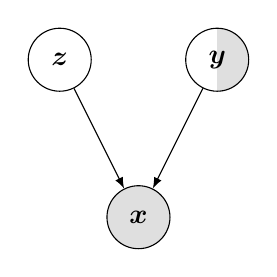
\begin{tikzpicture}
      \draw node at (0, 0) [place] (z) {$\vec{z}$};
      \draw node at (2, 0) [place] (y) {$\vec{y}$};
      \draw node at (1, -2) [place] (x) {$\vec{x}$};

      \begin{scope}[on background layer]
        \fill[fill=gray!25] (x.0) arc [start angle=0, end angle=360, radius=4mm];
        \fill[fill=gray!25] (y.270) arc [start angle=270, end angle=450, radius=4mm];
      \end{scope}

      \draw [->] (z) to (x);
      \draw [->] (y) to (x);
    \end{tikzpicture}
    \caption{The generative model}
  \end{subfigure}
  \begin{subfigure}[b]{0.4\linewidth}
    \centering
    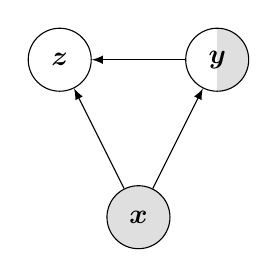
\begin{tikzpicture}
      \draw node at (0, 0) [place] (z) {$\vec{z}$};
      \draw node at (2, 0) [place] (y) {$\vec{y}$};
      \draw node at (1, -2) [place] (x) {$\vec{x}$};

      \begin{scope}[on background layer]
        \fill[fill=gray!25] (x.0) arc [start angle=0, end angle=360, radius=4mm];
        \fill[fill=gray!25] (y.270) arc [start angle=270, end angle=450, radius=4mm];
      \end{scope}

      \draw [->] (x) to (y);
      \draw [->] (x) to (z);
      \draw [->] (y) to (z);
    \end{tikzpicture}
    \caption{The inference model}
  \end{subfigure}
  \caption[Semi-supervised VAE]{The semi-supervised VAE \\ (shading indicates whether a variable is found in the dataset)}
  \label{fig:digit}
\end{figure}

In the semi-supervised model there are two inference cases. When the data is labelled the question is of how to infer $z$ from $x$ and $y$.
Despite $x$ and $y$ being marginally independent, they are not necessarily conditionally independent, and so both are used as input to
the encoder. Another reason for this is that it helps the encoder to learn to separate the representation of $y$ and $z$, so that $z$ contains
no information about the label. The semi-supervised VAE in this project uses a Gaussian distribution as the tractable distribution for 
$z$ (like the unsupervised VAE), and the encoder models $q(z|x, y)$ with a network $q_{\theta}(z|x, y)$. For labelled data the model should 
maximise the evidence $p(x, y)$, the probability the model assigns to the real data. This leads to a variant of the ELBO by marginalizing
out $z$:
\begingroup
\allowdisplaybreaks
\begin{align*}
  \log p(x, y) & = \log \int p(x, y, z) dz \\
  & = \log \int p(x|y, z)p(y)p(z) dz \qquad \text{Independence of $z$ and $y$}\\
  & = \log \int p(x|y, z)p(y)p(z) \frac{q(z|x, y)}{q(z|x, y)} dz\\
  & = \log\left(\mathbb{E}_q \left[\frac{p(x|y, z)p(y)p(z)}{q(z|x, y)}\right]\right) \\
  & \geq \mathbb{E}_q \left[\log\frac{p(x|y, z)p(y)p(z)}{q(z|x, y)}\right] \\
  & = \mathbb{E}_q \left[\log p(x|y, z) + \log p(y) + \log\frac{p(z)}{q(z|x, y)}\right] \\
  & = \mathbb{E}_q [\log p(x|y, z) + \log p(y)] - D_{KL}(q(z|x, y)||p(z)) \\
  & = -\mathcal{L}(x, y)
\end{align*}
\endgroup

This is very similar to the ELBO for the normal VAE, except that there is now a prior over $y$. This encodes previous knowledge about the 
distribution of the classes $y$, penalizing the model more when the label is of a low probability class. This is unimportant for the labelled
data as the previous knowledge is drawn from this data, but becomes important for the unlabelled data, and the connection between the two can be 
seen in the derivation below. A good model maximises the ELBO and therefore minimises $\mathcal{L}(x, y)$, which is used as the loss function.

When the data is unlabelled the problem is of inferring both $y$ and $z$ from $x$, $q(y, z|x)$. The evidence in the unlabelled case is $p(x)$,
and the ELBO can be derived by marginalizing out both $y$ and $z$:
\begingroup
\allowdisplaybreaks
\begin{align*}
  \log p(x) & = \log \sum_{y} \int p(x, y, z) dz \\
  & = \log \sum_{y} \int p(x, y, z) \frac{q(z, y|x)}{q(z, y|x)} dz\\
  & = \log \sum_{y} \int p(x, y, z) \frac{q(z|x, y)q(y|x)}{q(z|x, y)q(y|x)} dz\\
  & \geq \sum_{y} q(y|x) \int q(z|x, y) \log\frac{p(x, y, z)}{q(z|x, y)q(y|x)} dz \qquad \text{Jensen's inequality}\\
  & = \sum_{y} q(y|x) \int q(z|x, y) \log\frac{p(x, y, z)}{q(z|x, y)} dz - \sum_{y} q(y|x) \log q(y|x) \int q(z|x, y) dz\\
  & = \sum_{y} q(y|x)(-\mathcal{L}(x, y)) + \mathcal{H}(q(y|x)) \\
  & = -\mathcal{U}(x, y)
\end{align*}
\endgroup

The marginalization of $y$ is done by summation because the labels are discrete. Looking at the penultimate line of the derivation there is
the term $q(y|x)$. This is classification, inferring $y$ from $x$. This classifier is parameterised
by a neural network, and outputs a categorical distribution over the labels using the softmax function \eqref{softmax}. The summation term 
this is part of is referred to as ``classification as inference'' by Kingma~\cite{DBLP:journals/corr/KingmaRMW14}. For each label the labelled loss with 
respect to the data and that label is calculated and then multiplied by the probability of the label. This means that if a particular label
leads to a bad reconstruction, implying that the label was incorrect, and the classifier assigns a high probability to that (likely incorrect) label, 
the loss to the classifier will be very high, and minimizing this loss should lead to better classification. The prior over $y$ in $\mathcal{L}(x, y)$
becomes important here as it discourages the classifier from assigning a high probability to an unlikely class too often. All of this means that 
the classifier can learn directly from unlabelled data, with the small amount of labelled data providing a guide to good reconstructions.

The pipeline for labelled and unlabelled data is therefore slightly different at the moment. Labelled data is fed directly into the encoder
along with its label, and the loss function $\mathcal{L}(x, y)$ is calculated and backpropagated through the network. Unlabelled data is 
first put through the classifier, before it is fed into the encoder once with each label allowing $\mathcal{U}(x)$ to be computed and 
backpropagated through the network.

This means that at no point does the classifier learn directly from the labelled data, unnecessarily disadvantaging the model. To remedy
this the labelled loss function is modified to include an extra term, the cross entropy loss \eqref{eq:ce} between the real label and the 
label the classifier outputs for the data. This modified version is then:
\begin{align}
  \mathcal{J}(x, y) = \mathcal{L}(x, y) - \alpha (y \cdot \log q(y|x))
\end{align}

$\alpha$ is a hyperparameter that controls the weighting of the supervised loss, and is configured depending on the amount of labelled and 
unlabelled data available.

The model can now learn to classify from both labelled and unlabelled data at the same time, and so does not require pretraining the way
the previous models did.

\subsection{The ladder network} \label{ladder}

The ladder network is the most recent of the models included in this project having first been described by Valpola in 2014
~\cite{DBLP:journals/corr/Valpola14}, and then expanded upon by Rasmus et al. in 2015~\cite{DBLP:journals/corr/RasmusVHBR15}. 
It can be thought of as building on top of the SDAE, using an unsupervised local denoising 
criterion in order to improve the supervised performance of a deep feedforward network by using unlabelled data. However, instead of 
training each layer with its own denoising autoencoder, it instead adds a single deep decoder of the same size as the supervised network 
to the model, with lateral connections with trainable weights between the equivalent layers in the encoder and decoder.

\begin{figure}[H]
  \centering
  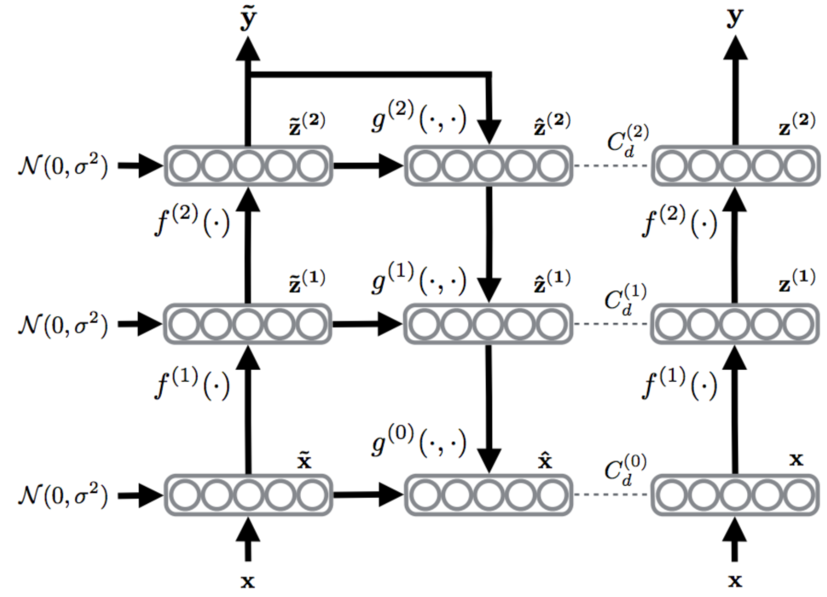
\includegraphics[scale=0.25]{figs/ladder.png}
  \caption[Illustration of the ladder network]{Illustration of the ladder network \\ (Source: Rasmus et al.~\cite{DBLP:journals/corr/RasmusVHBR15})}
  \label{fig:ladder}
\end{figure}

As described by Valpola, the ladder network is a form of hierarchical latent variable model. These differ from the latent variable models
looked at so far (autoencoder, VAE) in that they attempt to represent the data using hierarchies of latent variables. The model contains
layers of latent variables, with the higher layers describing \textit{some} of the variance of lower layers by $p(z^{(l)}|z^{(l+1)})$ ($z^{(0)} = x$). 
In a normal autoencoder the single latent layer $z$ has to encode everything about the data $x$, otherwise the reconstruction it generates 
will be very poor. With a hierarchical model each layer models some information about $x$, with the higher level latent variables 
(further from the data) able to be more abstract, as they don't have to encode the lower level details encoded in the previous (lower) layers. For example, using MNIST $z$ in a simple
autoencoder cannot just be the digit label as this does not provide enough information to reconstruct the original image well. In a hierarchical latent variable model the highest
level latent variable is able to be very abstract and only encode the label, as the other layers in the model provide less abstract information that can lead to a good reconstruction.
The reason this works in the ladder network is due to the lateral connections, which "leak" information from layers in the encoder to the decoder. This means that each decoder layer
receives information both from the previous decoder layer and the corresponding encoder layer. The encoder layer passes some information which
the subsequent encoder layers then no longer have to model.

This structure with the representation becoming more abstract in higher level layers is also analagous to how supervised learning works, with the layers 
further into the network modelling more complicated and abstract features with the final layer just outputting a class label (most abstract). For example in convolutional
neural networks (used extensively in vision), visualisation of the feature maps learned in image classification tasks have shown they are hierarchical. The lower layers
have high spatial resolution for detecting low-level features like edges and the higher layers have lower spatial resolution but can capture more abstract and complex features
(like people)~\cite{conv_hierarch}.

At the input to each decoder layer $u^{(l)}$ the corresponding encoder representation $z^{(l)}$ and the output of the previous decoder layer $u^{(l+1)}$ are combined together
using a combinator function $g$. $g$ has trainable parameters, but this leads to a problem where the lowest possible unsupervised MSE loss \eqref{eq:mse} can be 
achieved by $g$ learning to copy $z^{(l)}$ and completely ignoring the $u^{(l+1)}$, which corresponds to copying the input directly to the output at the bottom layer.
This completely short circuits the autoencoder, and in order to prevent this, Gaussian noise (sampled from $\mathcal{N}(0, 1))$) is added to the input to each layer 
in the encoder. Each encoder layer then has the representation $\tilde{z}^{(l)}$ and this noise means that just copying over the input no longer minimises the cost function. 

However if the unsupervised cost function used is simply the reconstruction loss between $\hat{x}$ and $x$ the first layer of the network still has a disproportionate
influence on the loss. In order to remedy this Valpola proposes adding local denoising criterion. This involves adding a cost function at each layer of the decoder,
namely the MSE~\eqref{eq:mse} between $g(\tilde{z}^{(l)}, u^{(l+1)})$, which is $\hat{z}^{(l)}$, a denoised representation of $\tilde{z}^{(l)}$, and $z^{(l)}$, the clean 
representation from layer $l$ of the encoder. In order to generate both the clean and noisy encoder representations the encoder is run twice per training iteration,
once without the added noise to generate $z^{(l)}$, and once with noise to generate $\tilde{z}^{(l)}$. These local cost functions require all the layers to learn in order
to make a meaningful representation that can be denoised well. Each layer loss is multiplied by a hyperparameter $\lambda_{l}$ according to how important the denoising cost
of the layer is, before being summed together to give a final unsupervised cost function per sample of:

\begin{align}
  \mathcal{U}(x) = \sum_{l} |z^{(l)} - \hat{z}^{(l)}|^{2}
\end{align}

The model as explained so far allows the ladder network to learn abstract features in the higher layers. However, without supervised data and a supervised cost function the 
features learned are unlikely to be useful for the classification task. The small amount of labelled data is used as a guide for this. The encoder of the model is the 
original classifier so the data is passed through the encoder and cross entropy loss~\eqref{eq:ce} is computed between the output and the labels. During training noise is 
added at the output of each layer, the same as one run of supervised learning, as the noise acts as a regularizer~\cite{NoiseInj}.

While the illustration of the model (Fig.~\ref{fig:ladder}) makes it look like it has three networks, the first and third column are both the encoder, with the first being 
noisy and the second being clean. A final overview of the training process is then:
\begin{enumerate}
  \item Data is passed into the clean encoder and the output from each layer is saved.
  \item Data is passed through the noisy encoder, and output from each layer is saved.
  \item The final output from the noisy encoder is the classification output, and supervised loss is computed with it.
  \item The output from the noisy encoder is fed into the decoder. At each layer $l$ of the decoder $g(\tilde{z}^{(l)}, u^{(l+1)})$ is calculated,
        and the unsupervised loss for the layer is computed.
  \item The unsupervised losses are multiplied by hyperparameter $\lambda_{l}$ and summed together.
  \item The supervised and unsupervised losses are summed and backpropagated through the network and the weights are updated.
\end{enumerate}  

\section{Requirements analysis}

By taking the success criteria from the project proposal (Appendix ~\ref{proposal}) I constructed a set of tasks that must be completed for the 
project and ranked them by their priority. The success criteria are:

\begin{itemize}
  \item The implemented models achieve close to original paper performance on the MNIST dataset 
  \item The final chosen model achieves better prediction accuracy than supervised learning alone on genetic datasets
  \item A tool is built that takes in file paths to unlabelled and labelled data and trains a classifier based on this
\end{itemize}

The first success criteria differs from the project proposal. After reading the papers of the models to be implemented (Section~\ref{reading}) I 
realised that the most important models, the semi-supervised variational autoencoder and the ladder network, both had benchmarks given on 
the MNIST database of handwritten digits~\cite{lecun-mnisthandwrittendigit-2010}. As the stated aim of generating synthetic data was to
ensure that the models were working correctly, I decided that a better measure of the correctness of the models was whether they
achieved (close to) the accuracy reported in the papers.

The models compared in this project in order to decide on the best semi-supervised method to use were:

\begin{itemize}
  \item \textbf{A variant of the Kingma M1 model}~\cite{DBLP:journals/corr/KingmaRMW14}. A variational autoencoder trained on combined 
        labelled and unlabelled data followed by a neural network classifier trained on the latent representation of the labelled data.
  \item \textbf{A stacked denoising autoencoder}~\cite{Vincent:2010:SDA:1756006.1953039}.
  \item \textbf{A semi-supervised variational autoencoder}.~\cite{DBLP:journals/corr/KingmaRMW14} Also referred to as the Kingma M2 model.
  \item \textbf{A ladder network}~\cite{DBLP:journals/corr/RasmusVHBR15}
\end{itemize}

With these models selected and the success criteria defined above the requirements can be constructed:

\begin{table}[H]
  \label{tab:requirements}
  \small % text size of table content
  \centering % center the table
  \begin{tabular}{lccr} % alignment of each column data
  \toprule[\heavyrulewidth]\toprule[\heavyrulewidth]
  \textbf{Requirement} & \textbf{Priority} \\ 
  \midrule
  Implement simple multilayer perceptron & Medium \\
  Implement Kingma M1 model & Medium \\
  Implement stacked denoising autoencoder & Medium \\
  Implement semi-supervised autoencoder & High \\
  Semi-supervised autoencoder achieves close to original paper \\ accuracy on MNIST & Medium \\
  Implement ladder network & High \\
  Ladder network achieves close to original paper accuracy \\ on MNIST & Medium \\
  Process the Cancer Genome Atlas gene expression data & High \\
  Evaluate and compare performance of models on MNIST & Low \\
  Evaluate and compare performance of models on TCGA data & High \\
  Implement saliency for best performing model (extension) & Low \\
  \bottomrule[\heavyrulewidth] 
  \end{tabular}
  \caption{Requirements for a successful project} 
\end{table}

\section{Starting point and reading} \label{reading}

I had some previous knowledge about neural networks and machine learning techniques through completing \textit{Introduction to data science}
and \textit{Artificial intelligence I} as part of Part IB, and completing the machine learning course by Andrew Ng on Coursera. However,
I had no previous experience with autoencoders, semi-supervised learning or Bayesian inference, and also little experience of optimising 
a machine learning model. To this end I decided upon a list of essential reading:

\begin{itemize}
  \item Lecture slides for \textit{Machine learning and Bayesian inference} by Holden~\cite{ML_Bayes}
  \item \textit{Deep learning} by Goodfellow et al.~\cite{Goodfellow-et-al-2016}
  \item \textit{Auto-encoding variational Bayes} by Kingma et al.~\cite{DBLP:journals/corr/KingmaW13}
  \item \textit{Semi-supervised learning with deep generative models} by Kingma et al.~\cite{DBLP:journals/corr/KingmaRMW14}
  \item \textit{Stacked denoising autoencoders: learning useful representations in a deep network with a local denoising criterion} by 
        Vincent et al.~\cite{Vincent:2010:SDA:1756006.1953039}
  \item \textit{From neural PCA to deep unsupervised learning} by Valpola~\cite{DBLP:journals/corr/Valpola14}
  \item \textit{Semi-supervised learning with ladder networks} by Rasmus et al.~\cite{DBLP:journals/corr/RasmusVHBR15}
\end{itemize}

\section{Resources}

\subsection{Language and libraries}

I made the decision to use Python, as it has support for two of the most popular and intuitive deep learning libraries, PyTorch and 
Tensorflow. Both frameworks are computationally similar, using a tape-based automatic differentiation system for backpropagation, and a C/C++ 
engine for speed. After reading through an introduction to both languages, and looking at a comparison of the features offered I decided to 
use PyTorch, as it felt more flexible, allowing the user to easily stop and start training at any point, and allowing much easier access 
to intermediate variables for debugging. In Tensorflow all operations have to be run using a Session object, and the only variables a 
user can see are those returned from the session object. PyTorch seems to me to have better integration with Python, allowing the user to 
access all the variables in a model at any time. The training is also more intuitive in PyTorch, with all the calculations of the loss 
and backpropagation done within a for loop over the dataset. In Tensorflow the variable to optimise is defined before looping and the 
backpropagation is done automatically by the Session object.

I used the PyCharm IDE for writing my Python code as I was familiar with Jetbrains IDEs.
PyCharm includes useful features like autocomplete, and has good integration with git.

\subsection{Hardware}

All of the programming was done on my laptop (Macbook Pro 2014, 2.6 GHz Intel Core i5, with 8GB of RAM, a 128GB SSD and 128GB SD card).

Running the models, especially on the highly dimensional gene expression data, is extremely computationally intensive, and runs much 
quicker on a GPU. To this end I was given access to NVIDIA Titan X and P100 GPUs by Prof. Li\'o.

\subsection{Backing up}

To back up my project and dissertation files and code I stored them in a git repository synced with a remote repository on GitHub. I also 
made regular backups of my entire SSD to an external hard drive.

\section{Summary}

This section should have provided an overview of the theory behind this project, and of the requirements that must be completed to 
ensure the project is a success.

\chapter{Implementation}

\section{Dealing with data}

\section{Model and class structure}

\section{Hyperparameter optimisation}

\section{Pipeline}

\chapter{Evaluation}

\section{MNIST results}

\section{TCGA results}

\subsection{Missing data}

\subsection{Hyperparameters}

\section{METABRIC results}

\section{Saliency}

\chapter{Conclusion}

% \section{Verbatim text}

% Verbatim text can be included using \verb|\begin{verbatim}| and
% \verb|\end{verbatim}|. I normally use a slightly smaller font and
% often squeeze the lines a little closer together, as in:

% {\renewcommand{\baselinestretch}{0.8}\small
% \begin{verbatim}
% GET "libhdr"
 
% GLOBAL { count:200; all  }
 
% LET try(ld, row, rd) BE TEST row=all
%                         THEN count := count + 1
%                         ELSE { LET poss = all & ~(ld | row | rd)
%                                UNTIL poss=0 DO
%                                { LET p = poss & -poss
%                                  poss := poss - p
%                                  try(ld+p << 1, row+p, rd+p >> 1)
%                                }
%                              }
% LET start() = VALOF
% { all := 1
%   FOR i = 1 TO 12 DO
%   { count := 0
%     try(0, 0, 0)
%     writef("Number of solutions to %i2-queens is %i5*n", i, count)
%     all := 2*all + 1
%   }
%   RESULTIS 0
% }
% \end{verbatim}
% }

% \section{Tables}

% \begin{samepage}
% Here is a simple example\footnote{A footnote} of a table.

% \begin{center}
% \begin{tabular}{l|c|r}
% Left      & Centred & Right \\
% Justified &         & Justified \\[3mm]
% %\hline\\%[-2mm]
% First     & A       & XXX \\
% Second    & AA      & XX  \\
% Last      & AAA     & X   \\
% \end{tabular}
% \end{center}

% \noindent
% There is another example table in the proforma.
% \end{samepage}

% \section{Simple diagrams}

% Simple diagrams can be written directly in \LaTeX.  For example, see
% figure~\ref{latexpic1} on page~\pageref{latexpic1} and see
% figure~\ref{latexpic2} on page~\pageref{latexpic2}.

% \begin{figure}
% \setlength{\unitlength}{1mm}
% \begin{center}
% \begin{picture}(125,100)
% \put(0,80){\framebox(50,10){AAA}}
% \put(0,60){\framebox(50,10){BBB}}
% \put(0,40){\framebox(50,10){CCC}}
% \put(0,20){\framebox(50,10){DDD}}
% \put(0,00){\framebox(50,10){EEE}}

% \put(75,80){\framebox(50,10){XXX}}
% \put(75,60){\framebox(50,10){YYY}}
% \put(75,40){\framebox(50,10){ZZZ}}

% \put(25,80){\vector(0,-1){10}}
% \put(25,60){\vector(0,-1){10}}
% \put(25,50){\vector(0,1){10}}
% \put(25,40){\vector(0,-1){10}}
% \put(25,20){\vector(0,-1){10}}

% \put(100,80){\vector(0,-1){10}}
% \put(100,70){\vector(0,1){10}}
% \put(100,60){\vector(0,-1){10}}
% \put(100,50){\vector(0,1){10}}

% \put(50,65){\vector(1,0){25}}
% \put(75,65){\vector(-1,0){25}}
% \end{picture}
% \end{center}
% \caption{A picture composed of boxes and vectors.}
% \label{latexpic1}
% \end{figure}

% \begin{figure}
% \setlength{\unitlength}{1mm}
% \begin{center}

% \begin{picture}(100,70)
% \put(47,65){\circle{10}}
% \put(45,64){abc}

% \put(37,45){\circle{10}}
% \put(37,51){\line(1,1){7}}
% \put(35,44){def}

% \put(57,25){\circle{10}}
% \put(57,31){\line(-1,3){9}}
% \put(57,31){\line(-3,2){15}}
% \put(55,24){ghi}

% \put(32,0){\framebox(10,10){A}}
% \put(52,0){\framebox(10,10){B}}
% \put(37,12){\line(0,1){26}}
% \put(37,12){\line(2,1){15}}
% \put(57,12){\line(0,2){6}}
% \end{picture}

% \end{center}
% \caption{A diagram composed of circles, lines and boxes.}
% \label{latexpic2}
% \end{figure}



% \section{Adding more complicated graphics}

% The use of \LaTeX\ format can be tedious and it is often better to use
% encapsulated postscript (EPS) or PDF to represent complicated graphics.
% Figure~\ref{epsfig} and~\ref{xfig} on page \pageref{xfig} are
% examples. The second figure was drawn using \texttt{xfig} and exported in
% {\tt.eps} format. This is my recommended way of drawing all diagrams.


% \begin{figure}[tbh]
% \centerline{
\includegraphics{figs/cuarms.pdf}}
% \caption{Example figure using encapsulated postscript}
% \label{epsfig}
% \end{figure}

% \begin{figure}[tbh]
% \vspace{4in}
% \caption{Example figure where a picture can be pasted in}
% \label{pastedfig}
% \end{figure}


% \begin{figure}[tbh]
% \centerline{\includegraphics{figs/diagram.pdf}}
% \caption{Example diagram drawn using \texttt{xfig}}
% \label{xfig}
% \end{figure}

% \section{Printing and binding}

% Use a ``duplex'' laser printer that can print on both sides to print
% two copies of your dissertation. Then bind them, for example using the
% comb binder in the Computer Laboratory Library.

% \section{Further information}

% See the Unix Tools notes at

% \url{http://www.cl.cam.ac.uk/teaching/current-1/UnixTools/materials.html}

% I hope that this rough guide to writing a dissertation is \LaTeX\ has
% been helpful and saved you time.


%%%%%%%%%%%%%%%%%%%%%%%%%%%%%%%%%%%%%%%%%%%%%%%%%%%%%%%%%%%%%%%%%%%%%
\addcontentsline{toc}{chapter}{Bibliography}
\printbibliography
% %%%%%%%%%%%%%%%%%%%%%%%%%%%%%%%%%%%%%%%%%%%%%%%%%%%%%%%%%%%%%%%%%%%%%
% % the appendices
% \appendix

% \chapter{Latex source}

% \section{diss.tex}
% {\scriptsize\verbatiminput{diss.tex}}

% \section{proposal.tex}
% {\scriptsize\verbatiminput{proposal.tex}}

% \chapter{Makefile}

% \section{makefile}\label{makefile}
% {\scriptsize\verbatiminput{makefile.txt}}

% \section{refs.bib}
% {\scriptsize\verbatiminput{refs.bib}}

\newpage

\appendix

\chapter{Backpropagation} \label{backprop}

Backpropagation is the flow of information from the outputs of the network back through the network. Once the cost function has been computed
finding the gradient of the loss with respect to each trainable parameter shows which direction the parameter can be shifted to decrease 
the loss function.. This derivation of the backpropagation algorithm is based on that found in \textit{Artificial intelligence I}~\cite{Art_Int}.
In the derivations below:
\begin{itemize}
  \item $J(\vec{\theta})_k$ is the cost function for the $kth$ sample in the training set
  \item $w_{i \to j}$ is the weight between node $i$ and node $j$
  \item $a_j$ is the value computed by the node $j$ pre-activation ($\sum_{k} w_{k \to j} z_k$)
  \item $z_j$ and $y_j$ are the values post-activation ($\sigma(a_j)$), for non-output and output nodes respectively
\end{itemize}

The value to be calculated for each weight (per sample) is $\frac{\partial J(\vec{\theta})_k}{\partial w_{i \to j}}$. To do this we use the chain rule
of differentiation:
\begin{align}
  \frac{\partial J(\vec{\theta})_k}{\partial w_{i \to j}} & = \frac{\partial J(\vec{\theta})_k}{\partial a_j} \frac{\partial a_j}{\partial w_{i \to j}} \\
  & = \frac{\partial J(\vec{\theta})_k}{\partial a_j} z_i
\end{align}

Then for weights connected to the output nodes:
\begin{align}
  \frac{\partial J(\vec{\theta})_k}{\partial w_{i \to j}} & = \frac{\partial J(\vec{\theta})_k}{\partial a_j} z_i \\
  & = \frac{\partial J(\vec{\theta})_k}{\partial y_j} \frac{\partial y_j}{\partial a_j} z_i
\end{align}

If our loss function is differentiable with respect to $y_j$, and $y_j$ is differetiable with respect to $a_j$ then we can calculate this.  
For backpropagation to work all our loss and activation functions must have this property. Thankfully all the loss and activation functions 
shown in this dissertation do have that property and so work correctly with backpropagation.

Once the gradients are computed for the weights in the output layer it is possible to calculate them for the next layer, and then the
layer after that, etc., as the errors are backpropagated through the network. The computation for the hidden layers is slightly more 
complicated:
\begin{align}
  \frac{\partial J(\vec{\theta})_k}{\partial w_{i \to j}} & = \frac{\partial J(\vec{\theta})_k}{\partial a_j} z_i \\
  & = \left( \sum_{k \in K} \frac{\partial J(\vec{\theta})_k}{\partial a_k} \frac{\partial a_k}{\partial a_j} \right) z_i
\end{align}
\begin{center}
  \textit{where K is the set of all nodes $j$ is connected to in the next layer}
\end{center}

By definition:
\begin{align}
  \frac{\partial a_k}{\partial a_j} & = \frac{\partial}{\partial a_j} \left( \sum_{i} w_{i \to k} z_i \right) \\
  & = \frac{\partial}{\partial a_j} \left( \sum_{i} w_{i \to k} \sigma(a_i) \right) \\
  & = w_{j \to k} \sigma'(a_j)
\end{align}

Therefore, for hidden layers:
\begin{align}
  \frac{\partial J(\vec{\theta})_k}{\partial w_{i \to j}} & = \left( \sum_{k \in K} w_{j \to k} \frac{\partial J(\vec{\theta})_k}{\partial a_k} \right) \sigma'(a_j) z_i
\end{align}

As the errors are moving backward through the network, and all nodes $k$ are in the layer after $j$, $\frac{\partial J(\vec{\theta})_k}{\partial a_k}$
has already been computed and so this gradient can be calculated.

\chapter{The reparameterization trick} \label{reparam}

It is not possible to backpropagate the reconstruction loss of a varitaional autoencoder through the random sampling in the latent dimension, because the drawing of
the samples is not differentiable with respect to $\vec{\mu}$ and $\vec{\sigma}$. Previously this was solved using a Monte Carlo gradient estimator, but these have 
extremely high variance and are impractical.Instead the reparameterization trick allows the Gaussian sample to be reparameterized as:
\begin{align}
  \vec{z_{i}} = \vec{\mu} + \vec{\sigma}\vec{\epsilon}
\end{align}

$\vec{\epsilon}$ is a vector of samples from the standard normal distribution $\mathcal{N}(0, 1)$. The sampling operation is now differentiable
with respect to $\vec{\mu}$ and $\vec{\sigma}$ and therefore is differentiable with respect to $\vec{\theta}$, the trainable parameters of the encoder. As the
gradients can be backpropagated through the network it is possible to train the VAE using gradient descent.

\chapter{Project Proposal} \label{proposal}
% Note: this file can be compiled on its own, but is also included by
% diss.tex (using the docmute.sty package to ignore the preamble)
\documentclass[12pt,a4paper,twoside,openany]{article}
\usepackage[pdfborder={0 0 0}]{hyperref}
\usepackage[margin=25mm]{geometry}
\usepackage{graphicx}
\usepackage{parskip}

\begin{document}

\begin{center}
\Large
Computer Science Tripos -- Part II -- Project Proposal\\[4mm]
\LARGE
A tool for phenotype prediction from cell genotype

\large
C.~London, Trinity College

Originator: Prof P.~Li\'o \& H.~Andres~Terre

19 October 2018
\end{center}

\vspace{5mm}

\textbf{Project Supervisor:} Prof P.~Li\'o \& H.~Andres~Terre

\textbf{Director of Studies:} Prof F.~Stajano

\textbf{Project Overseers:} Prof J.~Daugman  \& Dr A.~Madhavapeddy

% Main document

\section*{Introduction}

Phenotype prediction from cell genotype is an important problem in the field of bioinformatics, with usages in agriculture (for selecting crops with highest yield potential), medicine (for predicting likelihood of diseases/mutations), research, and many other fields. With the decreasing cost of genome sequencing this is becoming far more feasible for use in both research and the private sector.

Deep learning techniques provide an opportunity for generating high accuracy predictions of the phenotype from the genotype and as such much research in this area uses techniques such as autoencoders and neural networks to attempt to do this. However, much of the state of the art research is focused on generating predictions for only one type of cell, and so the network is structured specifically towards this cell. This is then not generalisable and not useful in other scenarios.

This project aims to build a tool that will provide these high accuracy predictions and is generalisable to data from different cells. By providing genotype data tagged with the observed phenotype for training, a user should then be able to use this tool to predict the required phenotype.

\section*{Starting point}

\subsection*{Prior Research}

This project is based on similar state of the art work done in papers on DeepGS\cite{DeepGS} (genomic selection) and DeepMetabolism\cite{DeepMetabolism}.

DeepGS was used to predict several phenotypes (grain length, grain hardness, plant height and more for wheat) when given genomic markers, and is now available as an R library. However the method  uses convolution and sampling to reduce data dimensionality, whereas the DeepMetabolism uses unsupervised pre-training in the form of an autoencoder to speed the supervised learning up. I believe that this is the better way to do it, and prescribes a less rigid structure on the model.

DeepMetabolism was used to predict three phenotypes of \textit{Escherichia Coli} and uses unsupervised pre-training with an autoencoder. However the autoencoder is used for denoising purposes, and the output, a cleaned version of the input data, is used for predictio instead of using the latent representation. The autoencoder is also structured specifically to correspond to the genome and proteins of \textit{E. Coli} and so the re-usability is limited.

\subsection*{Libraries and codebase}

The code for the learning will be written in Python, because Python has excellent support for advanced deep learning libraries. I have written machine learning code in Python before using Scikit-learn, but for this project I will use either Tensorflow or PyTorch as these libraries provide much better support for deep learning applications, as well as allowing for data parallelism and therefore large speed-ups when running on a GPU.

\section*{Resources required}

For this project I shall mainly use my own laptop, a 2014 Macbook Pro with a dual core Intel i5, 8GB of RAM and 128GB of flash storage. Source code for the project will be kept in a Git repository that will be synced with a repository on Github. The \LaTeX\\ source will be stored on my machine, and backed up to both overleaf.com and Google Drive. The entire content of my laptop will be frequently backed up to an external 500GB HDD.

The training of the model will be done using GPUs that can be provided by the Computer Lab, with confirmation from Professor Li\'o.

Data for training and testing the model will be both artificially generated as part of the project, and provided by the Plant Sciences department.

\section*{Work to be done}

\subsection*{Reading and further research}

\begin{itemize}
    \item Re-read papers on DeepGS and DeepMetabolism looking for particular insight into the exact models used to see ways they could be improved.
    
    \item Deep learning to model the hierarchical structure of the cell[3] - this is less relevant to the project as it involves a neural network that is pre-structured by hand, but still involves genotype-phenotype prediction and so may contain useful insights.
    
    \item Principles of gene manipulation and genomics\cite{Genomics} Chapters 16 to 20 - a book about genome analysis, involving genomic and transcriptomic data. This is necessary because I have never worked on a project with large scale genome analysis before.
    
    \item Reducing the dimensionality of data using neural networks\cite{Encoders} - information on reducing the dimensionality of data using autoencoders.
    
    \item Sparse autoencoders (lecture notes by Andrew Ng) - more information about using autoencoders to learn the most important features of data unsupervised.
    
    \item Meetings with Prof. Haseloff - Prof. Haseloff is a member of the plant sciences department here at the university and has experience working with the Computer Lab on other bioinformatics projects. He should be able to provide real data to use in training, as well as insight into what the synthetic data should look like.
    
\end{itemize}

\subsection*{The model}

The model for predicting the phenotype will be split into unsupervised and supervised portions.

The unsupervised portion is used to for dimesionality reduction of data, and is effectively a sort of pre-training for the model. Genomic data can be very large depending on the cell and so reducing the dimensionality to only the most important features should significantly speed the model up, and should hopefully provide greater prediction accuracy. This pre-training is likely to involve passing the genomic data into an autoencoder. An autoencoder is made up of two parts, an encoder and a decoder. The encoder includes the input layer and some hidden layers culminating in a final layer that has fewer nodes than the input layer. This layer is the latent representation of the input data. The decoder then attempts to reconstruct the input data from this representation, and backpropagation is performed to get the reconstruction as close as possible to the original. This latent representation should then be the features of the data that are most important for accurate reconstruction, and is therefore a reduced dimensionality representation of the data.

The supervised portion of the model will take the form of a neural network that takes in this latent representation as input and outputs the predicted phenotype. Backpropagation is performed to train the network to accurately predict the phenotype.

An important feature of the model should be the ability to work with different sized inputs and outputs. For the model to be generalisable to different cells, it will have to be able to take variable sized genome inputs, as the length of a genome sequence varies greatly between organisms. The output size will also not always be constant as the phenotype can take many forms - sometimes it might simply be a number e.g. if the studied phenotype is plant height, whereas other times it could be a class, or, as written in the extensions below, a photograph.

\paragraph{Testing.}

Testing the model will first be done with synthetic data, to ensure that it is working as it should i.e. recognising patterns and correctly identifying the most important features in the data, and the phenotype that should be associated with a given latent representation. The generation of this synthetic data will form an early part of this project, and will be done with input from Prof. Haseloff as he has significant experience with biological data.  

Once this is completed the model will then be trained and tested on real world data to verify its accuracy and usefulness as a real world prediction tool.

\subsection*{The tool}

This project should lead to a tool that can be used to predict phenotype without requiring users to know much about the underlying machine learning. To that end the tool should provide a basic front-end where users can add a file with training data, and, once training has completed, provide data that they want predictions for. The difficulty here is dealing with the different phenotypes a user might want, and having a model that can handle very different output requirements.

\section*{Success criteria}

Evaluation of the success of the project will be based upon the following criteria:

\begin{itemize}
    \item Better prediction accuracy than supervised training alone on a synthetic dataset (generated as part of the project) - compare the predicted phenotype with the synthetic phenotype generated for a particular pattern in the synthetic genotype data.
    \item Better prediction accuracy than supervised training alone on real world genotype and phenotype data.
    \item Producing a tool with a front-end that takes a file-path and trains the model based on the data within the file.
\end{itemize}

Prediction accuracy can be compared using a statistical significance test. The models will be trained on the same dataset and then tested on data that was not part of the training set. With synthetic data it is easy to generate data that was not part of the training set. With real world data if there is not enough for a separate training set and test set k-fold cross-validation can be performed.

\section*{Possible extensions}

If the main result is achieved and time is left some possible extensions are:

\begin{itemize}
    \item Use images of a cell/plant/etc. as the phenotype for training, and generate images as predictions. This would involve using other deep learning techniques to generate the images, likely generative adversarial networks.
    
    \item Measuring the importance of inputs to the output. Neural networks are often considered to be a sort of black box where input goes in and a result comes out. It is possible however to use some techniques to discover the importance of the input to the result. This can then be used to pinpoint which genes were most responsible for a certain phenotype. However, results can be misleading and the accuracy is not always good.
    
    \item Autoencoder structure based upon cell structure. Some well-studied organisms have extensive prior knowledge about gene interactions available in resources such as the Gene Ontology which would enabling structuring the autoencoder such that it partially mimics the cell. This should speed up training and could increase prediction accuracy. It would not be available for all cells, but if a user was using a well-studied cell the option to use a structured autoencoder would be useful.
\end{itemize}


\section*{Timetable}

Planned starting date is 20/10/2018.

\begin{enumerate}

\item \textbf{20/10/2018 -- 3/11/2018 } 

Perform the reading and research as stated in the "Work to be done" section. Install Tensorflow and PyTorch and decide which to use by doing small example learning tasks.

\item \textbf{4/11/2018 -- 18/11/2018} 

Write Python code to generate synthetic data for training. Begin building unsupervised model. Begin writing Introduction and Preparation chapters of dissertation.

\item \textbf{19/11/2018 -- 3/12/2018} 

Train and tune unsupervised model on synthetic data. Ensure that features expected to be important have large impact. Begin building supervised model. Begin writing Implementation chapter of dissertation.

\item \textbf{Michaelmas vacation} 

Do supervised training using output from the unsupervised model as input to the network. Make sure model is generalisable to different sized inputs and outputs corresponding to different cells and phenotypes.

\textbf{Milestones:}
\begin{itemize}
    \item Have a working prediction model trained on the synthetic data.
    \item Have finished writing dissertation Introduction and Preparation chapters.
\end{itemize}

\item \textbf{15/01/2019 -- 29/01/2019} 

Write progress report. Compare accuracy of model against a simple supervised model on artificial data to ensure model has better accuracy. Begin writing Evaluation chapter of dissertation.

\item \textbf{30/01/19 -- 13/02/19} 

Train model on real data and compare prediction accuracy with only supervised network.

\textbf{Milestones:}
\begin{itemize}
    \item Progress report submitted on 01/02/19.
\end{itemize}

\item \textbf{14/02/19 -- 28/02/19} 

Build a front-end that allows a user to pass a file of training data and create a model. Begin Extension 1: using images as phenotype.

\textbf{Milestones:}
\begin{itemize}
    \item Have a working tool allowing users to provide their own data for training.
    \item Have completed the Implementation chapter of the dissertation.
\end{itemize}

\item \textbf{01/03/19 -- 15/03/19} 

Extension 2: Pinpointing genes that have the greatest effect on phenotype.
Ensure full evaluation of all success criteria. Begin writing dissertation Evaluation chapter.

\item \textbf{Easter vacation}  

Writing dissertation and finishing any ongoing extensions. Extension 3 if time allows.

\item \textbf{23/04/19 -- 7/5/19} 

Proof reading, performing any final changes recommended by supervisor, preparing for submission in order to focus on exams.

\textbf{Milestone:} Have a completed and checked dissertation.

\end{enumerate}

\begin{thebibliography}{}
\bibitem{DeepGS} 
Ma W. \& Qiu Z. (2017) \textit{DeepGS: Predicting phenotypes from genotypes using Deep Learning}
\bibitem{DeepMetabolism}
Guo W., Xu Y. \& Feng X. (2017) \textit{DeepMetabolism: A Deep Learning System to Predict Phenotype from Genome Sequencing}
\bibitem{CellStructure}
Ma J., Yu M., Fong S., \& Ideker T. (2018) \textit{Using deep learning to model the hierarchical structure and function of a cell}
\bibitem{Genomics}
Primrose S. \& Twyman R. (2006) \textit{Principles of Gene Manipulation and Genomics}
\bibitem{Encoders}
Hinton G. \& Salakhutdinov R. (2006) \textit{Reducing the Dimensionality of Data with Neural Networks}

\end{thebibliography}

\end{document}

\end{document}
